% !TEX spellcheck = en_US

% !TEX root = elastophi-report.tex

\section*{Introduction}

This document aims at presenting the work achieved for project Elasto$\Phi$ during the CEMRACS summer school  
that took place at the Centre International de Rencontres Math\'ematiques (CIRM) at Luminy from July 25th to 
August 25th, 2016. This project originated from mathematical challenges encountered by IFP Energies Nouvelles (IFPEN)
for the numerical solution of an elastostatic problem in an infinite homogeneous background medium containing crack 
networks with highly complex geometrical structure, see Figure~\ref{fig:structureExamples}. 

\begin{figure}[hb]
\centering
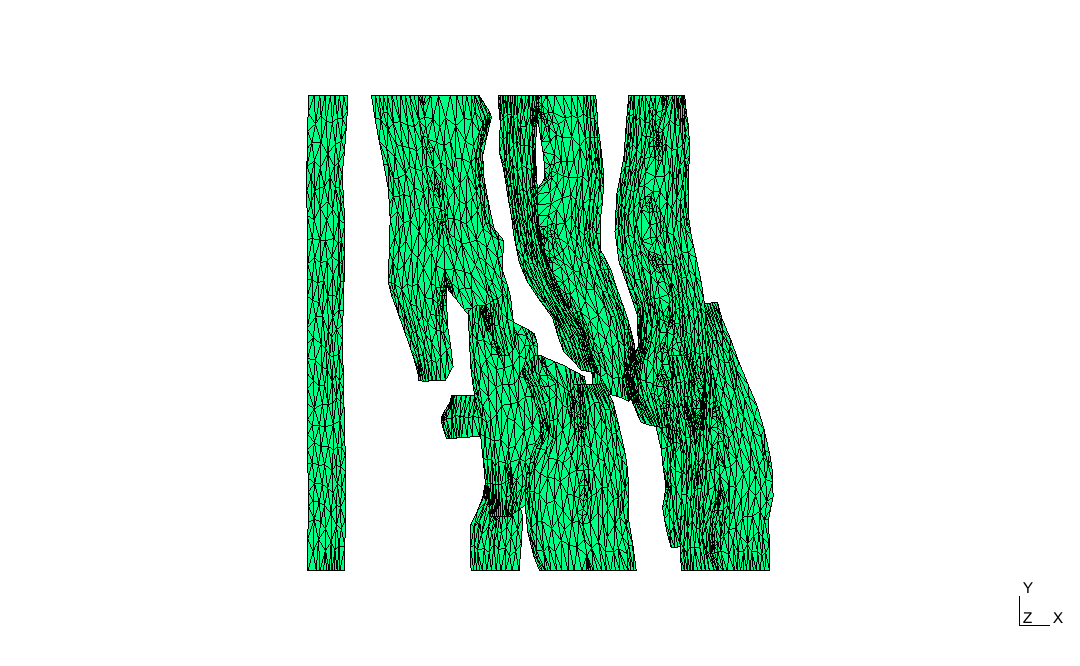
\includegraphics[width=0.4\textwidth]{../images/visu_maillage5364FracsTriangles.png} \quad
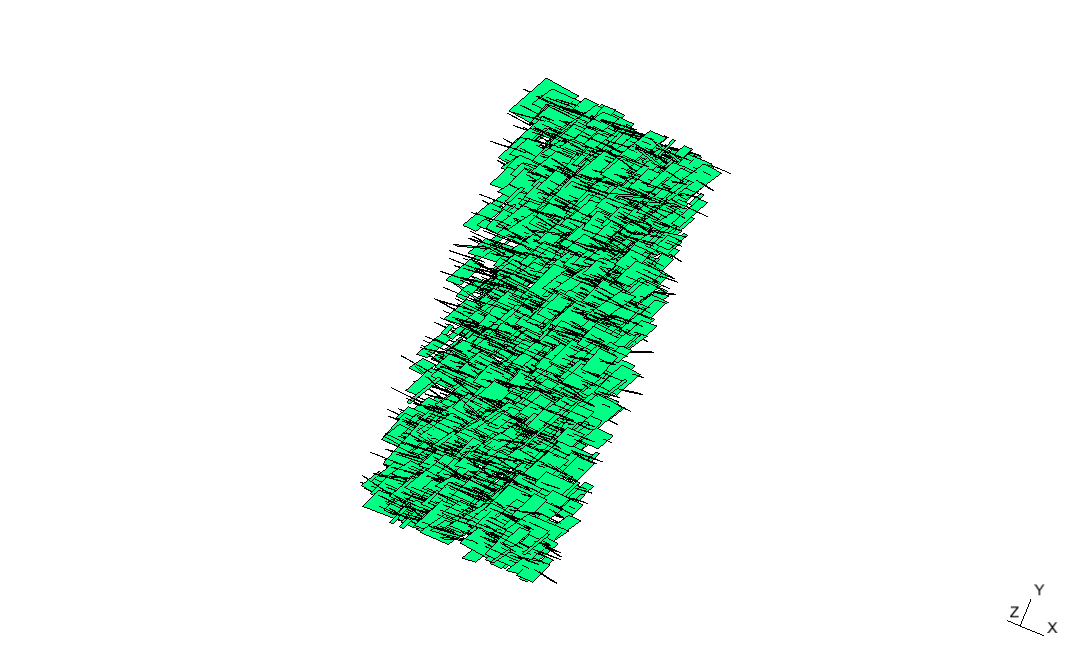
\includegraphics[width=0.3\textwidth]{../images/visu_maillage1994Fracs.png}
\caption{Examples of crack networks: fault network (left) and discrete fracture network (right).}
\label{fig:structureExamples}
\end{figure}

\bigskip
This problem was reformulated as boundary integral equation posed at the surface of cracks, and 
discretized by means of Galerkin procedure based on piecewise constant functions, which is commonly known as 
Boundary Element Method (BEM). The fully non-local structure of boundary integral operators leads to  
densely populated matrices. As a consequence, if the matrix of the problem is of size $N$, 
then any matrix-vector product (which is the most elementary building block of any iterative linear solver)
requires at least $\mathcal{O}(N^{2})$ operations.

\bigskip
As in most industrial applications, for the problems considered by IFPEN this situation is not acceptable. 
Indeed, computational complexity of $N^{2}$ makes it impossible to perform a matrix-vector product for $N$ larger than
say $10^{6}$: this would be too costly in terms of time and memory storage. At the same time, the  applications 
considered by IFPEN typically require $N$ to be of this order.

\bigskip
To deal with this difficulty, IFPEN developed a heuristic method consisting in forcing coefficients of the 
BEM matrix to zero whenever this coefficient corresponds to the interaction between sufficiently distant points 
of the crack network. With this procedure, the matrix of the problem is approximated by a sparsified matrix that 
allows matrix-vector products with $\mathcal{O}(N)$ complexity. But this strategy also induces substantial consistency 
error: measured in Frobenius norm, the perturbation on the matrix is typically between $16$\% and $40$\% large.

\bigskip
On the other hand, current literature on boundary integral equation nowadays offers a panel of refined complexity reduction 
techniques: fast multipole methods, hierarchical matrix strategies, and the like. These techniques, that have been developed 
during the last two decades, have been introduced to accelerate computations in a wide variety of problems ranging from molecular 
dynamics \cite{BOARD199289}, to astrophysics \cite{BarnesHut}. For a general overview see e.g.~\cite{Greengard}. Acceleration of 
boundary integral equations on smooth surfaces has also been historically a key challenge for stimulating the development of 
such methods \cite{MR805870}.

\bigskip
The main goal of the CEMRACS project Elasto$\Phi$ was to test the performance of one of these reduction techniques on the 
crack network problem of IFPEN. Although the above mentioned complexity reduction techniques are particularly well suited  
for boundary integral equations, the problem under consideration from IFPEN was not just a straightforward application of 
the state of the art, because it involves a strongly irregular geometry. Besides development issues, this was the main 
challenging  aspect of the project.

\bigskip
The Elasto$\Phi$ project mainly consisted in developing a numerical mockup code in C++ and testing it on the matrices sent 
by IFPEN. We implemented one particular complexity reduction technique: Hierarchical Matrix \cite{Hackbusch2016} format combined with the Adaptative Cross 
Approximation (ACA) compression method \cite{Bebendorf2008}. For the sake of brevity, we shall refer to this approach as HM-ACA. 
%We could not test several 
%complexity reduction techniques, this would have required more time (CEMRACS is only 5 weeks long\dots). 
Among all complexity reduction techniques 
already available (multipoles, panel clustering, etc\dots), we chose HM-ACA because this was the only approach that treats generation 
of the matrix of the problem in a black-box manner. All other methods are far more intrusive, and most of the time their development 
is also more time consuming. Besides, due to confidentiality restrictions, we did not have access to the source code of IFPEN, and 
in particular could not actually get the routine generating the matrix of the discretized problem. These constraints led us to choose HM-ACA.

\bigskip
There already exist freely accessible libraries written in C or C++ that implement HM-ACA, see e.g.~HLib (\url{http://hlib.org/}), H2Lib 
(\url{http://www.h2lib.org/}) or Ahmed (\url{https://github.com/xantares/ahmed}). But IFPEN required 
that the code numerical mockup developed during the project can be reused by IFPEN after the CEMRACS summer school, 
and the license of all existing libraries was incompatible with this condition. For these reasons, we decided to redevelop 
a "homemade" implementation of HM-ACA. The code that we developed was put under Lesser Gnu Public License (LGPL) and 
put on a GitHub repository freely accessible at
\begin{center}
\url{https://github.com/xclaeys/ElastoPhi}.
\end{center}

\medskip
The outline of this report is as follows. We will first describe the Adaptative Cross Approximation method, and show its efficiency 
for the compression of dense matrices admitting fast decreasing singular values (such matrices shall be referred to in the sequel as admissible). 
Unfortunately the matrices generated by boundary element  methods (and in particular the matrices considered by IFPEN) do not have 
fast decreasing eigenvalues. We shall then comment on this point, describing the problem and the boundary integral equation 
considered by IFPEN. Since the ACA compression method is not directly applicable, we are led to decompose the matrix in sub-blocks, 
each of which is either small or admissible. To be efficient, such a decomposition has to follow certain rules, and in particular 
admit a hierarchical structure. Such a technique, that we shall then describe, is referred to as a "hierarchical matrix format". 
Then we shall give a detailed overview of the code developed during the project, and conclude the report by a series of test 
cases where we report the performances of our code.

